
% v2-acmsmall-sample.tex, dated March 6 2012
% This is a sample file for ACM small trim journals
%
% Compilation using 'acmsmall.cls' - version 1.3 (March 2012), Aptara Inc.
% (c) 2010 Association for Computing Machinery (ACM)
%
% Questions/Suggestions/Feedback should be addressed to => "acmtexsupport@aptaracorp.com".
% Users can also go through the FAQs available on the journal's submission webpage.
%
% Steps to compile: latex, bibtex, latex latex
%
% For tracking purposes => this is v1.3 - March 2012
\documentclass[prodmode,acmtecs]{acmsmall} % Aptara syntax
\usepackage[spanish,polish]{babel}
\usepackage[T1]{fontenc}
\usepackage{fancyvrb}
\usepackage{graphicx,hyperref}
\newcommand\cutout[1]{}


\usepackage[table]{xcolor}
\usepackage[utf8]{inputenc}
\usepackage[parfill]{parskip}
\usepackage{tabulary}
\PassOptionsToPackage{hyphens}{url}
\usepackage{hyperref}    
\usepackage[capitalize]{cleveref}


% Metadata Information
% !!! TODO: SET THESE VALUES !!!
\acmVolume{0}
\acmNumber{0}
\acmArticle{CFP}
\acmYear{0}
\acmMonth{0}

\newcounter{colstart}
\setcounter{page}{4}

\RecustomVerbatimCommand{\VerbatimInput}{VerbatimInput}%
{
%fontsize=\footnotesize,
fontfamily=\rmdefault
}


\newcommand{\UnderscoreCommands}{%\do\verbatiminput%
\do\citeNP \do\citeA \do\citeANP \do\citeN \do\shortcite%
\do\shortciteNP \do\shortciteA \do\shortciteANP \do\shortciteN%
\do\citeyear \do\citeyearNP%
}

\usepackage[strings]{underscore}



% Document starts
\begin{document}


\setcounter{colstart}{\thepage}

\acmArticle{CFP}
\title{\huge\sc SIGLOG Monthly 220}
\author{DAVID PURSER\affil{Max Planck Institute for Software Systems, Saarbr\"ucken}
\vspace*{-2.6cm}\begin{flushright}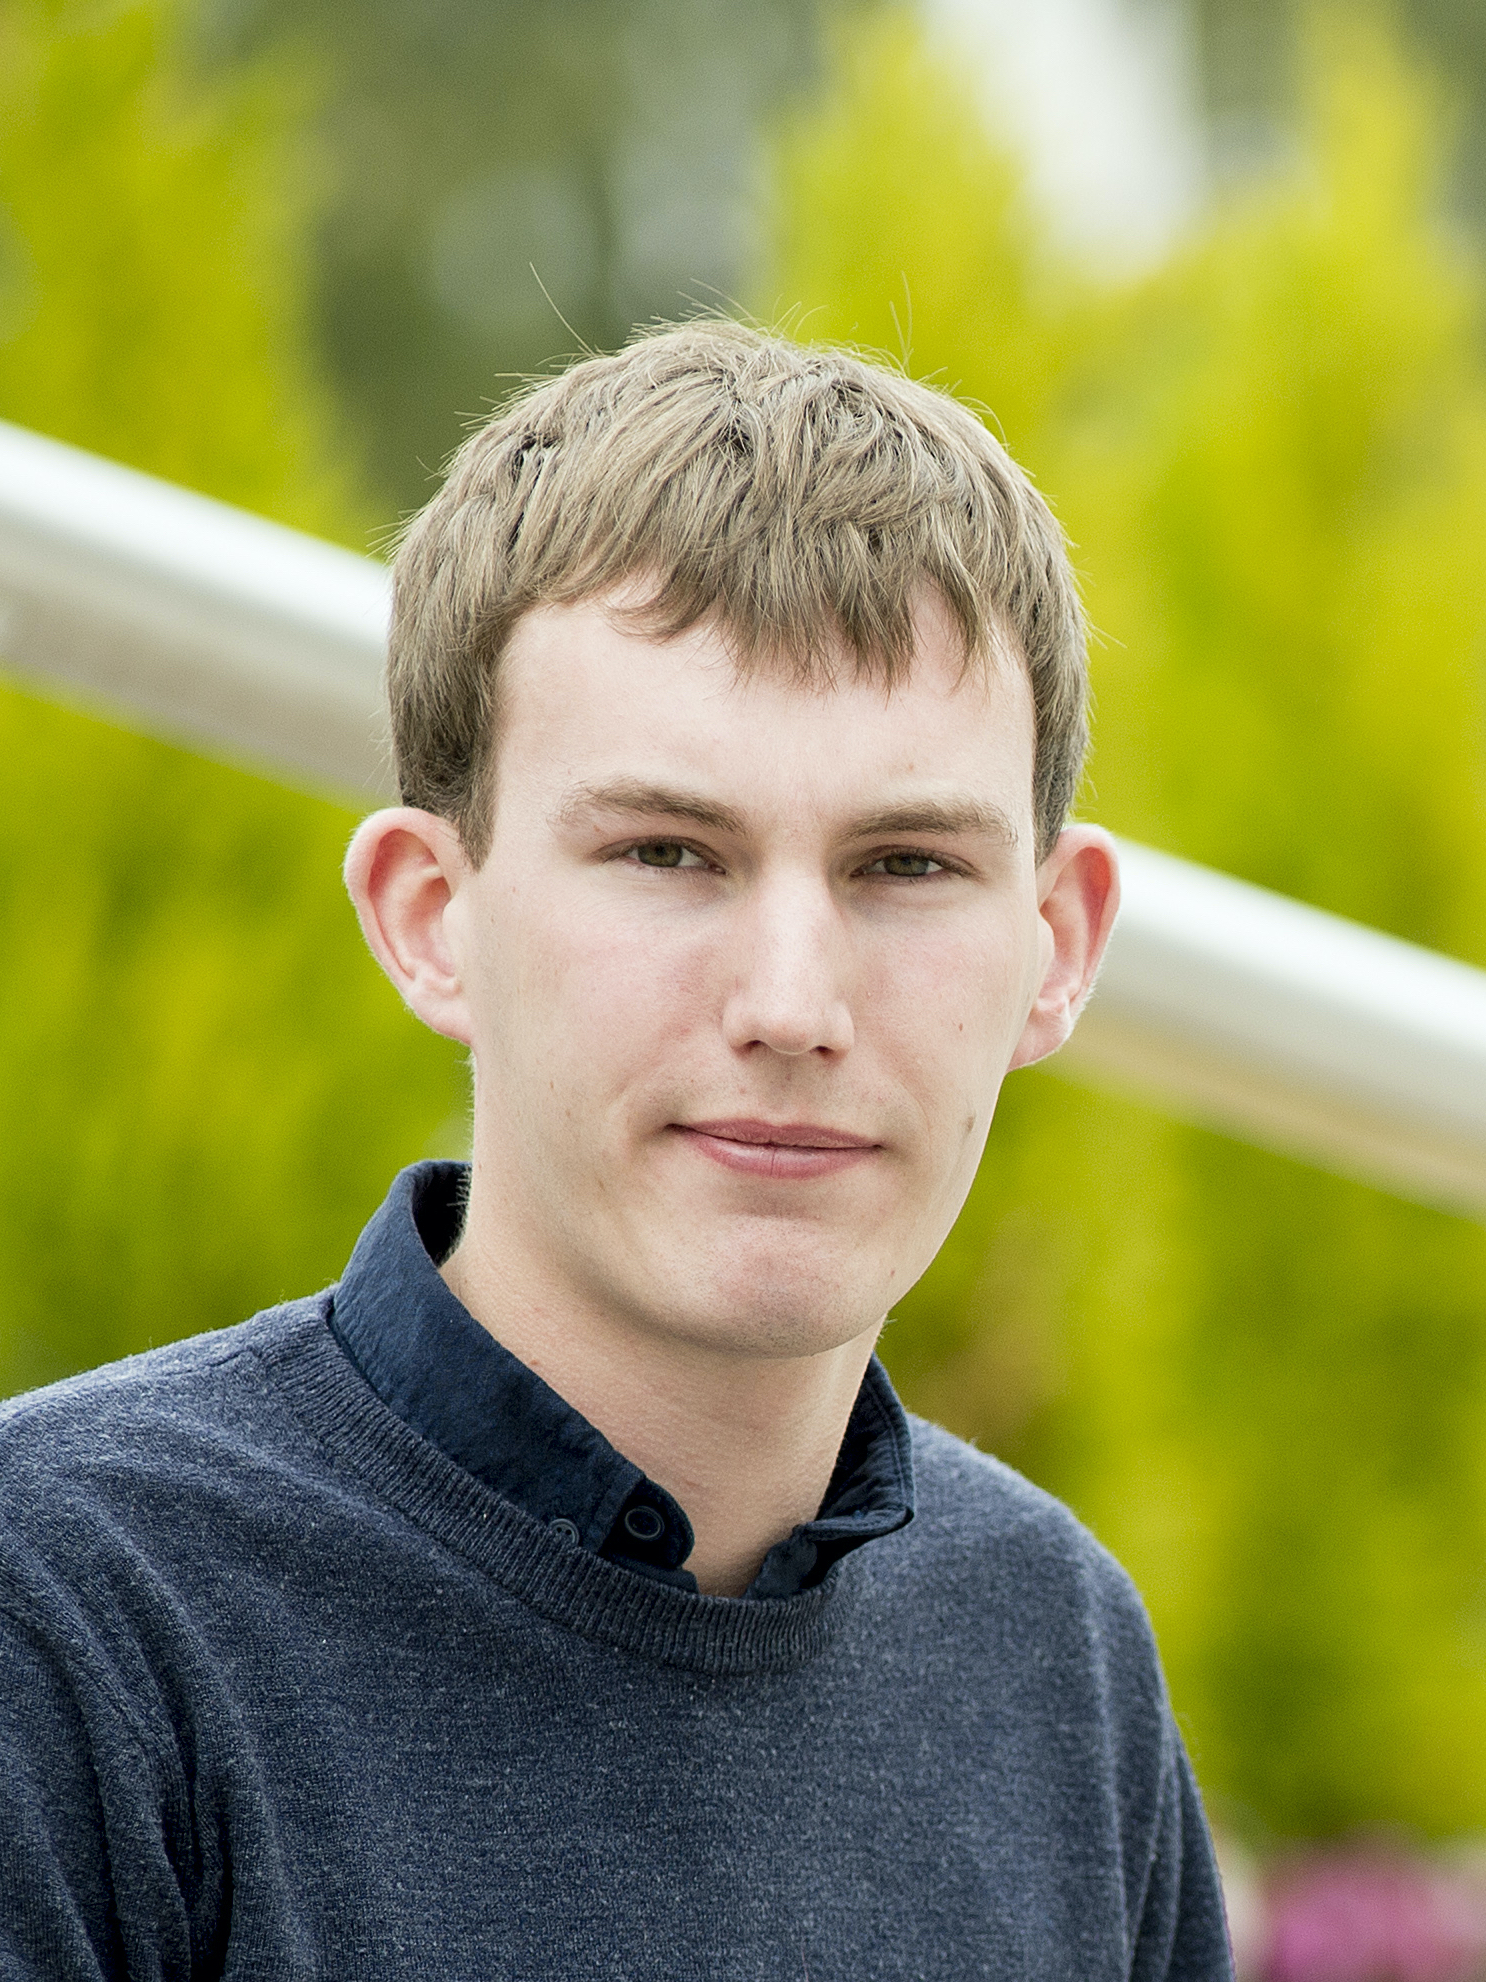
\includegraphics[width=30mm]{dp}\end{flushright}
}

\maketitlee

\href{https://lics.siglog.org/newsletters/}{Past Issues}
 - 
\href{https://lics.siglog.org/newsletters/inst.html}{How to submit an announcement}
\section{Table of Content}\begin{itemize}\item DEADLINES (\cref{deadlines}) 
 
\item ANNOUNCEMENTS 
 
\begin{itemize}\item Winners of the 2021 Ackermann Award (\cref{Winnersofthe2021AckermannAward})
\end{itemize} 
\item CALLS 
 
\begin{itemize}\item PODS 2022 (CALL FOR PAPERS) (\cref{PODS2022})
\item FoIKS 2022 (CALL FOR PARTICIPATION) (\cref{FoIKS2022})
\item TYPES 2022 and CA20111 (CALL FOR CONTRIBUTIONS) (\cref{TYPES2022andCA20111})
\end{itemize} 
\item JOB ANNOUNCEMENTS 
 
\begin{itemize}\item Research Positions available - working on Adaptive Cyber-Physical Systems at Mälardalen University, Sweden (\cref{ResearchPositionsavailableworkingonAdaptiveCyberPhysicalSystemsatMlardalenUniversitySweden})
\item Master in Pure and Applied Logic (\cref{MasterinPureandAppliedLogic})
\end{itemize} 
\end{itemize}\section{Deadlines}\label{deadlines}\rowcolors{1}{white}{gray!25}\begin{tabulary}{\linewidth}{LL}PODS 2022:  & Dec 10, 2021 (Second cycle abstract), Dec 17, 2021 (Full paper) \\
NFM 2022:  & Jan 03, 2022 (Abstract, EXTENDED), Jan 10, 2022 (Paper, EXTENDED) \\
CiE 2022:  & Jan 14, 2022 (Article registration, abstract), Jan 28, 2022 (Article) \\
LICS 2022:  & Jan 17, 2022 (Titles and Short Abstracts Due), Jan 21, 2022 (Full Papers Due) \\
CAV 2022:  & Jan 21, 2022 (Paper) \\
FSCD 2022:  & Jan 22, 2022 (Call for Locations), Feb 08, 2022 (Abstract), Feb 11, 2022 (Paper) \\
FoIKS 2022:  & Feb 04, 2022 (Abstract), Feb 11, 2022 (Paper) \\
AiML 2022:  & Mar 07, 2022 (Abstracts for full papers), Mar 14, 2022 (Full papers), May 23, 2022 (Short presentations) \\
TYPES 2022 and CA20111:  & Mar 09, 2022 (2 page abstract) \\
\end{tabulary}
\section{Winners of the 2021 Ackermann Award}\label{Winnersofthe2021AckermannAward}ANNOUNCEMENT 

\begin{itemize}\item  The Ackermann Award 2021, the EACSL Outstanding Dissertation Award for Logic in Computer Science, is given to two PhD theses (in alphabetic order) 
 
\begin{itemize}\item  Marie Fortin: Expressivity of first-order logic, star-free propositional dynamic logic and communicating automata
\item  Sandra Kiefer: Power and Limits of the Weisfeiler-Leman Algorithm
\end{itemize} 
\item  The award will be presented at the 30th Computer Science Logic (CSL 2022) Conference, the annual meeting of the European Association for Computer Science Logic. This will be held online, February 14th - 19th, 2022, organised by the Fundamentals of Computer Science Group at University of Göttingen, Germany. 
 
\item  A detailed report will be published in the proceedings of CSL 2022 
 
\end{itemize}\section{PODS 2022: 41st ACM SYMPOSIUM ON PRINCIPLES OF DATABASE SYSTEMS}\label{PODS2022}  Second Submission Cycle\\ 
  \href{https://databasetheory.org/node/125}{https://databasetheory.org/node/125}\\ 
CALL FOR PAPERS 

\begin{itemize}\item  SCOPE  
 
  PODS seeks high-quality scientific articles that present principled contributions to modeling, application, system building, and both theoretical and experimental validation in the context of data management. Such articles might be based, among others, on establishing theoretical results, developing new concepts and frameworks that deserve further exploration, providing experimental work that sheds light on the scientific foundations of the discipline, or a rigorous analysis of both widely used and recently developed industry artifacts. 
 
\item  CHANGES IN SUBMISSIONS:  
 
  There are two important changes with respect to submissions for PODS 2022. 
 
  1) Submitted papers must be formatted using the standard ACM proceedings stylesheet AND can be up to 8 pages. 
 
  2) For the first time, PODS 2022 will use a lightweight double-blind reviewing process. However, authors should feel free to disseminate their ideas or draft versions of their paper as they normally would. For instance, authors may post drafts of their papers on the web or give talks on their research ideas. 
 
\item  IMPORTANT DATES: Dates for the second submission cycle are as follows. 
 
\rowcolors{1}{white}{gray!25}\begin{tabulary}{\linewidth}{LL}Second cycle abstract:  & Dec 10, 2021 \\
Full paper submission:  & Dec 17, 2021 \\
Reviews sent to authors:  & Feb 28, 2022 \\
Rebuttal phase:  & Mar 1-5, 2022 \\
Notification:  & Mar 13, 2022 \\
\end{tabulary}
 
\end{itemize}\section{FoIKS 2022: 12th International Symposium on Foundations of Information and Knowledge Systems}\label{FoIKS2022}  University of Helsinki, Finland, Jun 20-23, 2022\\ 
  \href{https://foiks2022.github.io}{https://foiks2022.github.io}\\ 
CALL FOR PARTICIPATION 

\begin{itemize}\item  The FoIKS symposia provide a biennial forum for presenting and discussing theoretical and applied research on information and knowledge systems. The goal is to bring together researchers with an interest in this subject, share research experiences, promote collaboration, and identify new issues and directions for future research.  
 
  FoIKS 2022 solicits original contributions (as well as extensions of previously published contributions) dealing with any foundational aspect of information and knowledge systems. This includes submissions that apply ideas, theories or methods from specific disciplines to information and knowledge systems. Examples of such disciplines are discrete mathematics, logic and algebra, model theory, information theory, complexity theory, algorithmics and computation, statistics, and optimisation, among, of course, many others. 
 
  The FoIKS symposia are a forum for intensive discussions. Speakers will be given sufficient time to present their ideas and results within the larger context of their research. Furthermore, participants will be asked to prepare a first response to another contribution in order to initiate discussion. 
 
\item  SUGGESTED TOPICS 
 
  The suggested topics include, but are not limited to: 
 
\begin{itemize}\item  Database design: formal models, dependencies and independencies
\item  Big data: models for data in the Cloud, programming languages for big data, query processing
\item  Dynamics of information: models of transactions, concurrency control, updates, consistency preservation, belief revision
\item  Information fusion: heterogeneity, views, schema dominance, multiple source information merging, reasoning under inconsistency
\item  Integrity and constraint management: verification, validation, consistent query answering, information cleaning
\item  Intelligent agents: multi-agent systems, autonomous agents, foundations of software agents, cooperative agents, formal models of interactions, negotiations and dialogue, logical models of emotions
\item  Knowledge discovery and information retrieval: machine learning, data mining, formal concept analysis and association rules, text mining, information extraction
\item  Knowledge representation, reasoning and planning: non-monotonic formalisms, probabilistic and non-probabilistic models of uncertainty, graphical models and independence, similarity-based reasoning, preference modelling and handling, computational models of argument, argumentation systems
\item  Logics in databases and AI: classical and non-classical logics, logic programming, description logics, spatial and temporal logics, probability logic, fuzzy logic
\item  Mathematical foundations: discrete structures and algorithms, graphs, grammars, automata, abstract machines, finite model theory, information theory, coding theory, complexity theory, randomness
\item  Security in information and knowledge systems: identity thee, privacy, trust, intrusion detection, access control, inference control, secure Web services, secure Semantic Web, risk management
\item  Semi-structured data and XML: data modelling, data processing, data compression, data exchange
\item  Social computing: collective intelligence and self-organising knowledge, collaborative filtering, computational social choice, Boolean games, coalition formation, reputation systems
\item  The Semantic Web and knowledge management: languages, ontologies, agents, adaption, intelligent algorithms, ontology-based data access
\item  The WWW: models of Web databases, Web dynamics, Web services, Web transactions and negotiations, social networks, Web mining
\end{itemize} 
\item  SUBMISSION GUIDELINES 
 
\begin{itemize}\item  Long papers: suggested number of pages is 16, and the maximum number of pages is 18. 
\item  Short papers: the maximum number of pages is 10. 
\end{itemize} 
  All papers must PDF using LMCS LaTeX style, original and not simultaneously submitted to another journal or conference.  The submissions will be judged for scientific quality and for suitability as a basis for broader discussion. 
 
  Submission: \href{https://easychair.org/conferences/?conf=foiks2022}{https://easychair.org/conferences/?conf=foiks2022}  
 
\item  IMPORTANT DATES 
 
\rowcolors{1}{white}{gray!25}\begin{tabulary}{\linewidth}{LL}Abstract submission:  & Feb 04, 2022 \\
Paper submission:  & Feb 11, 2022 \\
Author notification:  & Apr 11, 2022 \\
Camera-ready paper due:  & May 06, 2022 \\
FoIKS 2022 Symposium:  & Jun 20-23, 2022 \\
\end{tabulary}
 
\item  PUBLICATION 
 
  The proceedings will be published by Springer-Verlag in the Lecture Notes in Computer Science. After the symposium, authors of selected papers will be invited to submit extended journal versions of their papers for a FoIKS 2022 special issue of the Annals of Mathematics and Artificial Intelligence or another journal. Exact details will be provided on the conference website in due time. 
 
\end{itemize}\section{TYPES 2022 and CA20111: 28th International Conference on Types for Proofs and Programs and EuroProofNet Cost Action meeting}\label{TYPES2022andCA20111}  Nantes, France,  Jun, 20-25 2022\\ 
  \href{https://types22.inria.fr}{https://types22.inria.fr}\\ 
CALL FOR CONTRIBUTIONS 

\begin{itemize}\item  BACKGROUND 
 
  The TYPES meetings are a forum to present new and on-going work in all aspects of type theory and its applications, especially in formalised and computer assisted reasoning and computer programming. 
 
  The TYPES areas of interest include, but are not limited to: 
 
\begin{itemize}\item  foundations of type theory and constructive mathematics;
\item  applications of type theory;
\item  dependently typed programming;
\item  industrial uses of type theory technology;
\item  meta-theoretic studies of type systems;
\item  proof assistants and proof technology;
\item  automation in computer-assisted reasoning;
\item  links between type theory and functional programming;
\item  formalizing mathematics using type theory.
\end{itemize} 
  We encourage talks proposing new ways of applying type theory. In the spirit of workshops, talks may be based on newly published papers, work submitted for publication, but also work in progress. 
 
  The EuroProofNet Cost Action CA20111 focuses on the same research topics as TYPES and partially sponsors the TYPES Conference. 
 
\item  CONTRIBUTED TALKS: 
 
  We solicit contributed talks. Selection of those will be based on extended abstracts/short papers of 2 pages (not including bibliography) formatted with easychair.cls. The submission site is \href{https://easychair.org/conferences/?conf=types2022}{https://easychair.org/conferences/?conf=types2022} 
 
\item  IMPORTANT DATES: 
 
\rowcolors{1}{white}{gray!25}\begin{tabulary}{\linewidth}{LL}2 page abstract submission:  & Mar 09, 2022 \\
notification of acceptance/rejection:  & Apr 20, 2022 \\
camera-ready version of abstract:  & May 15, 2022 \\
\end{tabulary}
 
  Camera-ready versions of the accepted contributions will be published in an informal book of abstracts for distribution at the workshop. 
 
\item  POST-PROCEEDINGS 
 
  A post-proceedings volume will be published in the Leibniz International Proceedings in Informatics (LIPIcs) series. Submission to that volume will be open to everyone. Tentative submission deadline for the post-proceedings: September 2022. 
 
\end{itemize}\section{Research Positions available - working on Adaptive Cyber-Physical Systems at Mälardalen University, Sweden}\label{ResearchPositionsavailableworkingonAdaptiveCyberPhysicalSystemsatMlardalenUniversitySweden}JOB ANNOUNCEMENT 

\begin{itemize}\item   At Mälardalen University in Sweden,  we have an extraordinary chance and a long-term plan to expand the department and hire competent researchers. Research Positions are announced to work on Adaptive Cyber-Physical Systems and their synthesis within the research lab for Cyber-Physical Systems Analysis. A PhD in Computer Science or Software Engineering is necessary. 
 
  For more information see the links below. 
 
\begin{itemize}\item  PostDoc Positions: The PostDoc Position has the condition of completion of the PhD degree not more than three years before the deadline. \href{https://web103.reachmee.com/ext/I018/1151/job?site=8\&lang=UK\&validator=2efd9e54ee423d53334ac7960e3b4e03\&job_id=1324}{https://web103.reachmee.com/ext/I018/1151/job?site=8\&lang=UK\&validator=2efd9e54ee423d53334ac7960e3b4e03\&job\_id=1324}
\item  More senior researchers are welcome to apply using this link: \href{https://web103.reachmee.com/ext/I018/1151/job?site=8\&lang=UK\&validator=2efd9e54ee423d53334ac7960e3b4e03\&job_id=1321}{https://web103.reachmee.com/ext/I018/1151/job?site=8\&lang=UK\&validator=2efd9e54ee423d53334ac7960e3b4e03\&job\_id=1321}
\end{itemize} 
Application deadline: Dec 15, 2021 
 
\item  Contact Person: Marjan Sirjani (marjan.sirjani@mdh.se, \href{http://www.es.mdh.se/staff/3242-Marjan_Sirjani}{http://www.es.mdh.se/staff/3242-Marjan\_Sirjani}) 
 
\end{itemize}\section{Master in Pure and Applied Logic }\label{MasterinPureandAppliedLogic}JOB ANNOUNCEMENT 

\begin{itemize}\item   The 2022--2024 edition of the two-year Master in Pure and Applied Logic jointly organized by the University of Barcelona (UB) and Polytechnical University of Catalunya (UPC) will soon open for pre-registration. Students are welcome to express their interest by sending their background, motivation, and CV to the email address masterlogic@ub.edu 
 
  The Master in Pure and Applied Logic caters in the most central aspects of advanced logic, including Computability Theory, Model Theory, Non-Classical Logics, Proof Theory and Set Theory. 
 
  Additional information on the master can be found at: 
 
\begin{itemize}\item  \href{http://www.ub.edu/masterlogic/}{http://www.ub.edu/masterlogic/}  
\item  \href{https://www.ub.edu/web/ub/en/estudis/oferta_formativa/master_universitari/fitxa/P/M0C0D/index.html}{https://www.ub.edu/web/ub/en/estudis/oferta\_formativa/master\_universitari/fitxa/P/M0C0D/index.html}? 
\item  \href{http://diposit.ub.edu/dspace/handle/2445/133559}{http://diposit.ub.edu/dspace/handle/2445/133559}
\end{itemize} 
  For questions related to eligibility, content, scheduling, scholarships, housing etc. please contact masterlogic@ub.edu 
 
\end{itemize}


To the \href{http://siglog.org/}{SIGLOG} or \href{https://lics.siglog.org}{LICS} website\end{document}